\begin{appendices}

\chapter{Mouckups de Interfaces del Sistema}
\label{anexo:mouckups}


% ------------------------------------------------------------------------------
% SECCIÓN 1: PERFIL QUEJOSO
% ------------------------------------------------------------------------------
\section{Perfil: Quejoso}
Este perfil corresponde a la comunidad politécnica (alumnos, docentes, administrativos). Las interfaces se centran en la accesibilidad y el seguimiento simple.

\begin{figure}[htbp]
    \centering
    % Asegúrate de que la ruta coincida con tu carpeta de imágenes
    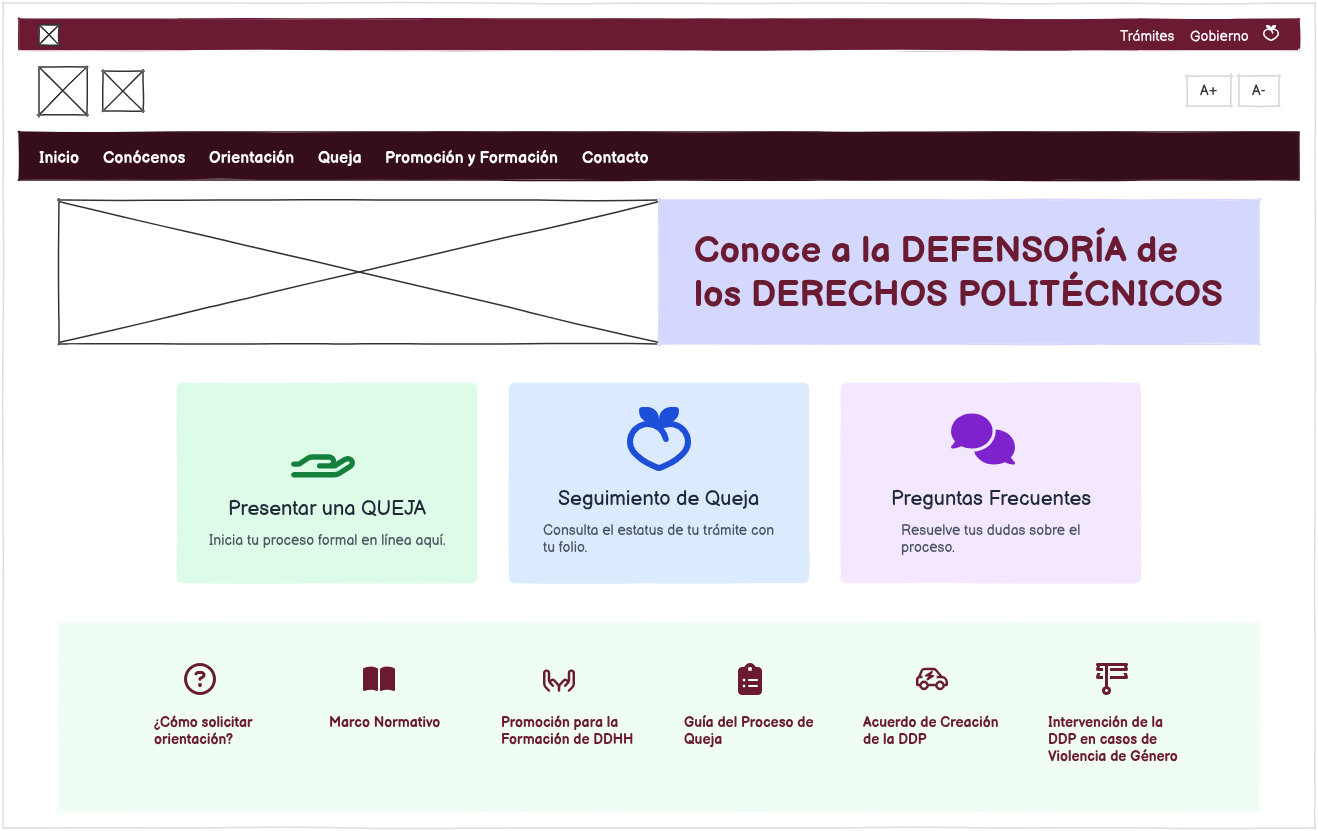
\includegraphics[width=1\textwidth]{imagenes/quejoso/Inicio.png}
    \caption{MQ-01: Pantalla de inicio y selección de trámite.}
    \label{fig:mq01_inicio}
    
    \vspace{0.5cm} % Espaciado entre la imagen y la descripción
    
    \begin{minipage}{0.95\textwidth}
        \small
        \textbf{Descripción de la interfaz:} \\
        La pantalla de inicio constituye el punto de entrada principal para el usuario. Presenta una arquitectura de información clara basada en la identidad institucional del IPN. Los elementos clave incluyen:
        \begin{itemize}
            \item \textbf{Menú de Navegación:} Acceso a secciones informativas como "Conócenos" y "Marco Normativo".
            \item \textbf{Accesos Directos:} Tres contenedores principales para "Presentar una QUEJA", "Seguimiento de Queja" (mediante folio) y "Preguntas Frecuentes".
            \item \textbf{Barra de Herramientas de Accesibilidad:} Ubicada en la parte superior derecha para ajustar el tamaño de fuente ($A+, A-$).
            \item \textbf{Footer Informativo:} Iconografía para acceso rápido a guías de proceso, normatividad y protocolos de violencia de género.
        \end{itemize}
    \end{minipage}
\end{figure}





\end{appendices}